% !TeX root = RJwrapper.tex
\title{crossfit: A Graph-Based Cross-Fitting Engine in R}


\author{by Etienne Peyrot and François Petit}

\maketitle

\abstract{%
Semiparametric procedures such as double/debiased machine learning (DML) use cross-fitting to evaluate targets with out-of-sample nuisance predictions. The crossfit package provides a general R engine in which users define a target functional and the nuisance models it requires. It executes an explicit schedule over folds and repeated data partitions, returning either a scalar estimate or a cross-fitted predictor function.
The package also supports nuisance dependency graphs, alternative allocations of training folds across nuisance components, and comparisons of several methods under shared splits. It reuses identical nuisance fits across methods and provides method-specific failure controls, which are useful in simulation studies and method development. Deterministic schedules and validation checks make the resulting cross-fitting procedure auditable. The package is available on CRAN and is openly developed on GitHub under GPL-3.
}

\textbf{Keywords:} cross-fitting; double machine learning; sample splitting; causal inference; semiparametric estimation; R

\section{Introduction}\label{sec:introduction}

\subsection{Cross-fitting and DML in brief}\label{subsec:primer}

Suppose the parameter of interest is a low-dimensional target \(\theta_0\), while its estimation also requires one or more nuisance functions collected in \(\eta_0\). Examples of nuisance functions include an outcome regression, a propensity score, or a data-dependent preprocessing rule. Flexible methods can reduce modeling restrictions for these functions, but evaluating a target with nuisance predictions fitted on the same observations can transmit overfitting bias to the target estimate.

Sample splitting separates these two operations: one part of the data is used to fit the nuisance functions, and a disjoint part is used to evaluate the target. Their roles are rotated over a \(K\)-fold partition. In the simplest case, this proceeds as follows:

\begin{enumerate}
\def\labelenumi{\arabic{enumi}.}
\tightlist
\item
  Divide the observations into \(K\) folds.
\item
  Fit the nuisance functions without one fold.
\item
  Predict the nuisance functions and evaluate the target on the held-out fold.
\item
  Repeat the fitting and evaluation steps until every fold has served as the held-out fold, then combine the fold-specific target estimates.
\end{enumerate}

Each observation therefore contributes to target evaluation through nuisance predictions obtained from fits that excluded that observation.

This approach has a long history in semiparametric statistics \citep{bickel1982, schick1986, zheng2011, newey2018}. It is a central component of Double/Debiased Machine Learning (DML) \citep{chernozhukov2018} and orthogonal statistical learning \citep{foster2023}. In these approaches, the target is commonly represented by a score \(\psi(W; \theta, \eta)\). Neyman orthogonality makes the expected score locally insensitive to small perturbations of the nuisance functions, while cross-fitting controls the dependence between nuisance estimation and score evaluation. Together, these properties permit flexible nuisance estimation while retaining valid inference under suitable regularity and rate conditions.

\subsection{Why a general cross-fitting engine is useful}\label{subsec:need}

The \texttt{crossfit} package is designed for settings where the cross-fitting scheme is itself part of the method to implement or study. The researcher defines the target and the nuisance quantities it requires, while the package organizes their fitting and out-of-sample evaluation. This separation is particularly useful for newly developed semiparametric estimators, for which the cross-fitting procedure would otherwise have to be implemented specifically for each estimator.

This focus differs from that of packages such as \texttt{DoubleML}, which provide complete estimation and inference procedures for established DML model classes \citep{bach2024}. \texttt{crossfit} instead exposes the cross-fitting construction itself. It can therefore accommodate estimators with several nuisance quantities, including settings where one nuisance depends on predictions from another or where different nuisance quantities must be fitted on different subsets of the available training data. These features are useful when the statistical properties of an estimator depend on how nuisance functions are trained relative to one another, for example when nuisance estimates should be based on separate training samples to limit dependence between their estimation errors.

The package is also intended for methodological comparisons and simulation studies. Competing estimators can be evaluated using the same random partitions, alternative ways of allocating training data among their nuisance functions can be compared without rewriting the estimator, and identical nuisance fits shared across methods can be computed only once. These capabilities, together with the need for reproducible cross-fitting schedules across large simulation studies and benchmarks of causal estimators, motivated the development of the package; preliminary versions were used in \citep{bouvier2024}.

For an estimator already covered by a \texttt{DoubleML} model class, \texttt{DoubleML} provides a direct route from nuisance estimation to inference. When the goal is instead to implement a researcher-defined cross-fitted estimator, control how its nuisance quantities are trained, or compare alternative cross-fitting designs under a common schedule, \texttt{crossfit} provides the corresponding general-purpose engine. The following example first illustrates its basic use before these additional controls are introduced.

\section{A first cross-fitting analysis}\label{sec:first-analysis}

Consider estimating the prediction error of a flexible regression method. With a two-fold split, the regression is fitted on the first fold and evaluated on the second. The roles of the folds are then reversed, and the two held-out errors are averaged. This simple procedure is a common cross-fitted estimation.

The example below follows the basic procedure used throughout the package: define a nuisance model, define the target, create a method specification, and run the schedule. The simulated outcome depends nonlinearly on \texttt{x}, and the nuisance regression is fitted with a random forest.

\begin{verbatim}
set.seed(123)
n <- 300
sim_data <- data.frame(x = runif(n, -2, 2))
sim_data$y <- sin(pi * sim_data$x) + rnorm(n, sd = 0.3)

nuis_y <- create_nuisance(
  fit = function(data) {
    ranger::ranger(y ~ x, data = data, num.trees = 100, seed = 1)
  },
  predict = function(model, data) {
    as.numeric(predict(model, data = data)$predictions)
  },
  train_fold = 1L
)

target_mse <- function(data, nuis_y, ...) mean((data$y - nuis_y)^2)

m <- create_method(
  target = target_mse,
  list_nuisance = list(nuis_y = nuis_y),
  folds = 2L,
  repeats = 1L,
  eval_fold = 1L,
  mode = "estimate",
  fold_allocation = "overlap",
  aggregate_panels = mean_estimate,
  aggregate_repeats = mean_estimate
)

res <- crossfit(sim_data, m, seed = 123)
res$estimate
\end{verbatim}

\begin{verbatim}
#> [1] 0.12092
\end{verbatim}

The target is evaluated twice, once for each held-out fold. The function supplied through \texttt{aggregate\_panels} averages these two mean squared errors. The same separation between evaluation data and nuisance fitting data is used when cross-fitting nuisance predictions for DML, although the target is then an orthogonal score rather than a prediction error.

A complete DML application to the partially linear regression model is provided in Appendix \hyperref[app:plr-pension]{DML for the partially linear regression model}.

\section{Package concepts and design}\label{sec:design}

The first analysis used the package's central objects. This section defines those objects and the schedule they produce.

\subsection{User-facing abstractions}\label{subsec:user-facing}

Two functions define the package's main objects.

\begin{itemize}
\tightlist
\item
  \textbf{\texttt{create\_nuisance()}} defines a nuisance node through a \texttt{fit()} function and a \texttt{predict()} function. Any fitting method that provides these two operations can be used, and \texttt{train\_fold} specifies how many folds train the node.
\item
  \textbf{\texttt{create\_method()}} combines a target functional with its named nuisances and the settings for data splitting, fold allocation, aggregation, and failure handling. A target is an R function with explicit nuisance arguments, such as \texttt{target(data,\ nuis\_y,\ nuis\_m)}.
\end{itemize}

Two output modes are supported. In \texttt{mode\ =\ "estimate"}, the target returns a numeric value. In \texttt{mode\ =\ "predict"}, it returns a prediction function for new data. Appendix \hyperref[app:predict]{Prediction mode} gives a complete example.

\subsection{Folds, panels, evaluation windows, and repetitions}\label{subsec:schedule}

The main notions introduced in this section, including folds, evaluation windows, and panels, are illustrated in Figure \ref{fig:terminology}. In \texttt{mode\ =\ "estimate"}, the data are first partitioned into \texttt{folds\ =\ K} subsets. The target is evaluated on an \textbf{evaluation window} which is a set of one or more consecutive folds. The argument \texttt{eval\_fold} gives the width of this window. Nuisance predictions supplied to the target are produced from fits whose training observations exclude the current evaluation window. Prediction mode instead uses \texttt{eval\_fold\ =\ 0}.

A \textbf{panel} is one position of the evaluation window in the cyclic schedule. With \texttt{K\ =\ 5} and \texttt{eval\_fold\ =\ 2}, the five panels evaluate on folds \((1,2)\), \((2,3)\), \((3,4)\), \((4,5)\), and \((5,1)\). The window advances by one fold between panels and wraps around after fold 5. The target is evaluated separately in each panel, giving the panel targets \(\widehat{\theta}^{(1)},\ldots,\widehat{\theta}^{(5)}\); the superscript indexes panels in Figure \ref{fig:terminology}.

\begin{figure}

{\centering 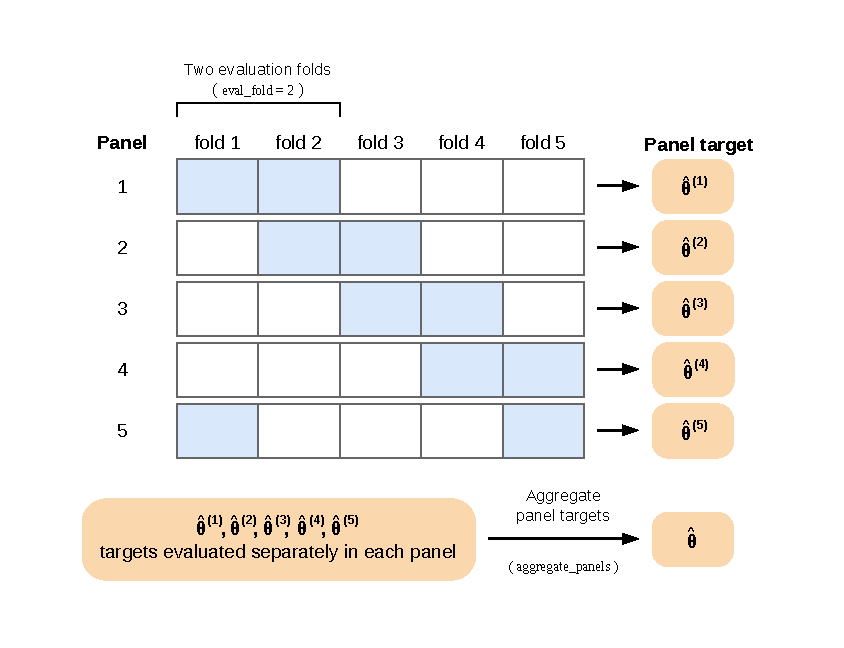
\includegraphics[width=\linewidth,alt={Diagram of a five-fold cross-fitting schedule. Five panel rows show a two-fold evaluation window moving cyclically across the folds, followed by panel-target aggregation.}]{figures/terminology} 

}

\caption{Schedule for five-fold cross-fitting with an \emph{evaluation window} width of two folds (\texttt{eval\_fold} = 2). Each row is a panel, and the highlighted \emph{evaluation window} advances cyclically by one fold. The target is evaluated separately in each panel, producing the panel targets shown with superscripts indexing panels. The function supplied through \texttt{aggregate\_panels} combines these panel targets. Unhighlighted folds lie outside the current \emph{evaluation window}; their use for nuisance training depends on \texttt{train\_fold} and \texttt{fold\_allocation}.}\label{fig:terminology}
\end{figure}

One \textbf{repetition} consists of one \(K\)-fold partition, the complete cycle of \(K\) panels, and aggregation of the corresponding panel targets. The split remains fixed throughout that cycle. The \texttt{repeats} argument specifies how many independently generated partitions are processed in this way.

\subsection{Aggregation over panels and repetitions}\label{subsec:aggregation}

Within each repetition, the target is evaluated separately in each of the \(K\) panels. The resulting panel-specific target values are then combined through \texttt{aggregate\_panels} to obtain one repetition-specific estimate. When \texttt{repeats\ \textgreater{}\ 1}, the data are partitioned again, the complete panel schedule is rerun, and another estimate is obtained. The function supplied through \texttt{aggregate\_repeats} then combines these repetition-specific estimates into the final value. The two aggregation functions are specified separately and need not be identical.

Using \texttt{repeats\ =\ 1} corresponds to ordinary \(K\)-fold cross-fitting and requires only one random partition. Repeating the splitting and aggregating the resulting estimates can reduce sensitivity to a particular random partition; Jacob \citep{jacob2020} illustrates this finite-sample benefit for heterogeneous treatment-effect estimators. Repeated splitting requires fitting the nuisance functions again, however, and no universal number of repetitions is recommended.

The package provides \texttt{mean\_estimate()} and \texttt{median\_estimate()} for numeric targets, and \texttt{mean\_predictor()} and \texttt{median\_predictor()} for prediction functions; custom aggregation functions may also be supplied. In \texttt{mode\ =\ "predict"}, the panel-specific and repetition-specific prediction functions are combined pointwise when called on new data.

\subsection{Reading the returned object}\label{subsec:first-result}

For one method, \texttt{crossfit()} returns the final value in the \texttt{estimate} component. The list \texttt{results\$values} contains the panel-aggregated value from each successful repetition before \texttt{aggregate\_repeats} is applied, while \texttt{results\$errors} records panel or aggregation errors. The remaining components report completed repetitions, fold requirements, the validated method, and the execution plan. Single-method results are not indexed by method name.

\subsection{Nuisance dependency graph and validation}\label{subsec:dag-validation}

Nuisance components form the nodes of a directed acyclic graph (DAG). A dependency arises when a nuisance's \texttt{fit()} or \texttt{predict()} function requires predictions from another nuisance component. The same representation covers data-dependent preprocessing, such as imputation, normalization, calibration, or feature construction. Before execution, the package validates nuisance graphs and method specifications:

\begin{itemize}
\tightlist
\item
  \textbf{Argument coverage checks:} required arguments in nuisance \texttt{fit()} and \texttt{predict()} functions must have corresponding nuisance mappings.
\item
  \textbf{Cycle detection:} cyclic dependency graphs are rejected early with informative errors.
\item
  \textbf{Target-nuisance consistency:} the target function's required nuisance arguments must be provided by the method specification.
\item
  \textbf{Input sanitization:} fold constraints, aggregation functions, failure controls, and mode-specific requirements are checked before execution.
\end{itemize}

These checks make invalid specifications explicit before the cross-fitting schedule begins.

\subsection{Fold allocation modes}\label{subsec:allocation}

All fold allocation modes in \texttt{crossfit} satisfy the same central requirement: in every mode, the target evaluation fold/window is disjoint from all nuisance training folds used to generate the nuisance predictions passed to the target. This is the usual out-of-sample guarantee targeted by standard DML cross-fitting \citep{chernozhukov2018, newey2018}.

\textbf{Allocation of training folds across nuisances.} Modes differ only in how training folds are assigned across nuisance instances inside a panel, that is, whether different nuisance models or branches of a nuisance dependency graph may reuse the same training folds.

This distinction matters because, beyond the leading orthogonality-driven cancellation, many doubly robust / orthogonal estimators have a remainder containing products of nuisance estimation errors. If nuisance errors are correlated because the nuisances were trained on the same data, this ``nonlinear'' term can behave poorly in finite samples. Several papers therefore consider strengthened splitting geometries that deliberately separate training samples across nuisance components. The terminology varies across the literature (``double cross-fitting'' \citep{newey2018, mcclean2024}, ``three-way cross-fitting'' \citep{fisher2023}, ``triple cross-fit'' \citep{ke2024}, and ``multiway cross-fitting'' \citep{chiang2022}) but the common principle is to train the nuisance components that interact in the remainder term on separate subsamples.

\textbf{The three allocation modes.} Figure \ref{fig:fold-allocation} shows the same method, represented by a triangle-shaped nuisance DAG, under the three modes for \texttt{K\ =\ 5}. It shows the panel in which the target is evaluated on fold 1 (blue); the other panels follow by cyclic shifts modulo \texttt{K}.

\begin{figure}

{\centering 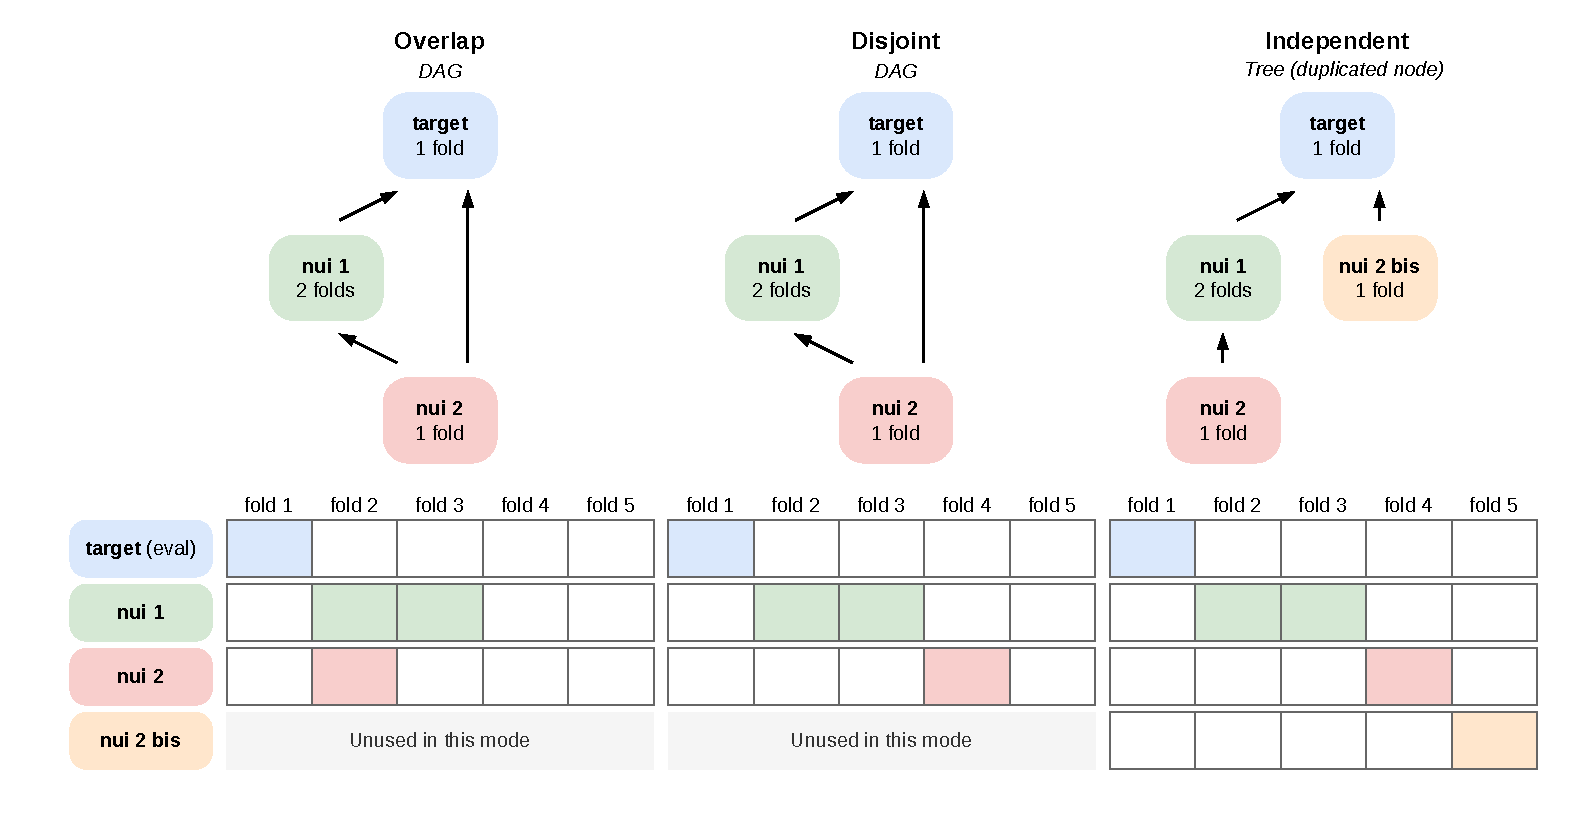
\includegraphics[width=\linewidth,alt={Diagram showing three fold allocation modes (overlap, disjoint, independence) for a small nuisance graph, with the evaluation fold highlighted and different training folds shown for each nuisance node.}]{figures/fold_allocation_modes} 

}

\caption{Fold allocation modes in crossfit. The same method is executed under three fold allocation modes. target denotes the user-defined target functional (the final quantity computed), and \texttt{nui 1}/\texttt{nui 2} denote two required nuisance models; the arrow \texttt{nui 2} \(\to\) \texttt{nui 1} indicates a nuisance-of-nuisance dependency. Top: nuisance dependency structure and node-specific training widths (\texttt{train\_fold} = number of folds used to train each nuisance). Bottom: for \texttt{K=5}, the panel where the target is evaluated on fold 1 (blue) is shown. Colored cells indicate the training folds used to fit each nuisance instance in that panel. \texttt{nui 2 bis} is a duplicated copy of \texttt{nui 2} used only in Independence mode.}\label{fig:fold-allocation}
\end{figure}

The modes differ as follows:

\begin{itemize}
\tightlist
\item
  \textbf{\texttt{"overlap"}} corresponds to the original, widely used cross-fitting geometry in DML. It enforces the out-of-sample constraint for the evaluation window, but allows different nuisances to use overlapping, often identical, training folds within a panel \citep{chernozhukov2018, newey2018}.
\item
  \textbf{\texttt{"disjoint"}} implements the central idea behind ``double'', ``triple'', and ``three-way'' designs in their simplest form. Within a panel, it coordinates training-fold assignment across nuisance instances to avoid fold reuse when possible, so nuisance models that jointly contribute to a second-order remainder term can be trained on different data \citep{mcclean2024, fisher2023, ke2024}. Shared nodes are not duplicated, so dependence can remain through an upstream fit that is used in several places.
\item
  \textbf{\texttt{"independence"}} applies a stronger separation. If a nuisance node is used in several branches, the engine duplicates that node by expanding the graph into a tree, allowing the branches to use disjoint training folds \citep{chiang2022}. This mode can require a larger \texttt{K} and more nuisance fits, but provides the strongest separation when a method uses the same nuisance in several places.
\end{itemize}

\textbf{Practical trade-offs.} Overlap mode corresponds to the default geometry in classical DML and is often a natural baseline \citep{chernozhukov2018}. Disjoint and independence modes control how much training data is shared across nuisance models. This connects to an active research question: when do stronger splitting geometries improve finite-sample performance by limiting dependence-driven second-order bias terms \citep{mcclean2024, fisher2023, ke2024, chiang2022, zivich2021}? The three modes permit these geometries to be compared without changing the target or nuisance definitions.

\subsection{Computation, reuse, and failure handling}\label{subsec:performance}

Nuisance fitting generally dominates the cost of simulation-heavy cross-fitting studies. The engine evaluates nuisance nodes in dependency order and reuses a fitted object only when the complete nuisance specification and its training-fold window are identical. Reuse is limited to one repetition because each repetition uses a new data partition.

When several methods are compared, \texttt{crossfit\_multi()} applies one schedule to all named method specifications in the call. The methods therefore use the same data partitions, and an identical nuisance request is fitted only once. Reuse is limited to structurally shared instances and nuisance nodes required in several places. Appendix \hyperref[app:multi]{Benchmarking multiple methods} gives a complete example.

The \texttt{"disjoint"} and \texttt{"independence"} allocation modes can introduce more nuisance instances than \texttt{"overlap"}. The cyclic panel schedule can nevertheless request the same instance more than once, so the number of graph nodes does not translate directly into the number of fits. Stronger allocation modes may also require a larger \texttt{K}, in which case the schedule contains more panels.

Errors are recorded separately for each method. Through \texttt{failure\_control}, a method specifies whether a panel error ends the current repetition, whether a previous failure of an identical shared fit prunes later work in that repetition, and how many failed repetitions are permitted. Other methods in the same \texttt{crossfit\_multi()} call continue according to their own controls.

Users may also supply a deterministic \texttt{fold\_split} function, enabling exact reproduction of fold schedules across machines and code revisions. The engine itself is sequential; higher-level parallelization is discussed in Section \hyperref[sec:discussion]{Discussion, limitations, and reuse}.

\section{Technical details and quality control}\label{sec:technical}

\subsection{Automated unit and integration testing}\label{automated-unit-and-integration-testing}

The automated test suite uses \texttt{testthat} (edition 3). Unit tests cover specification helpers (\texttt{create\_nuisance()}, \texttt{create\_method()}), aggregation utilities, and validation logic. Integration tests cover \texttt{crossfit()} and \texttt{crossfit\_multi()} in estimation and prediction modes.

\subsection{Cross-fitting invariants: no-leakage testing}\label{cross-fitting-invariants-no-leakage-testing}

Automated invariant tests verify that each nuisance prediction supplied to a target comes from a fit that excludes the corresponding evaluation fold. This check covers the \texttt{"overlap"}, \texttt{"disjoint"}, and \texttt{"independence"} allocation modes.

\subsection{Robustness: failure handling}\label{robustness-failure-handling}

Panel and aggregation errors are recorded separately for each method. By default, a panel error ends the current repetition. With \texttt{fail\_repetition\_on\_error\ =\ FALSE}, the remaining panels are evaluated and failed panels are passed as \texttt{NA\_real\_} to \texttt{aggregate\_panels}. The \texttt{max\_failed\_repetitions} setting controls when a repeatedly failing method is disabled, while other methods continue. The optional \texttt{prune\_on\_shared\_fit\_failure} setting skips a method when a structurally identical nuisance fit has already failed in the same repetition.

\subsection{Continuous integration}\label{continuous-integration}

GitHub Actions runs \texttt{R\ CMD\ check} on every push and pull request. Checks cover macOS and Windows with R release, and Ubuntu Linux with R release and R devel. This matrix reduces operating-system-specific regressions and tests compatibility with the next R release.

\section{Discussion, limitations, and reuse}\label{sec:discussion}

\subsection{Limitations and scope}\label{limitations-and-scope}

The package supplies cross-fitting rather than ready-made estimators. Its main limitations are:

\begin{itemize}
\tightlist
\item
  \textbf{No built-in estimators:} the package does not provide causal estimators, orthogonal scores, or standard-error formulas. Users define targets and inference procedures, and use the package to obtain cross-fitted nuisance predictions or target evaluations.
\item
  \textbf{Fold-geometry constraints:} stronger allocation modes such as \texttt{"disjoint"} and especially \texttt{"independence"} may require larger numbers of folds \texttt{K} (or may be infeasible for a given nuisance graph and node-specific \texttt{train\_fold} settings). They can also increase the number of nuisance instances to fit, trading statistical dependence reduction for additional computation.
\item
  \textbf{No internal parallelization:} the engine does not parallelize over folds, panels, or repetitions. Independent simulation replications or method grids can be parallelized outside a package call with standard R tools.
\item
  \textbf{User-defined code remains part of the analysis:} the schedule enforces out-of-sample fold separation, but nuisance functions should not use global state, retain data between calls, or access variables that should be unavailable at prediction time.
\end{itemize}

\subsection{Reuse potential}\label{reuse-potential}

The package can be used whenever estimation of a low-dimensional target requires out-of-sample nuisance predictions, including predictions from data-dependent preprocessing such as imputation. Examples include DML estimators for causal parameters, partially linear models, orthogonal-score-based targets, and procedures that require several dependent nuisance components. Because nuisances are defined through user-provided \texttt{fit()} and \texttt{predict()} functions, a wide range of R fitting methods can be used without imposing a particular model class.

\textbf{Prediction functions.} In addition to scalar target estimation, \texttt{mode\ =\ "predict"} constructs a function from cross-fitted nuisance predictions. This supports prediction on new data and methods that combine several cross-fitted prediction functions. Appendix \hyperref[app:predict]{Prediction mode} gives a complete example.

\textbf{Empirical methodology reuse.} The package is well-suited to simulation and benchmarking studies: users can vary \texttt{K}, repeated splitting, node-specific training widths, and fold-allocation modes to study finite-sample behavior under controlled schedules, including dependence-reduction geometries motivated by double, triple, and three-way cross-fitting \citep{mcclean2024, fisher2023, ke2024, chiang2022}. One repetition is the cheaper baseline; additional repetitions can be used when sensitivity to a random partition is itself relevant. The deterministic \texttt{fold\_split} interface supports reproducible experiments, including grouped or time-based splits when appropriate. As described in Section \hyperref[subsec:performance]{Computation, reuse, and failure handling}, \texttt{crossfit\_multi()} applies identical splits to competing methods and can reuse shared nuisance fits.

\subsection{Extending the software}\label{extending-the-software}

The core engine can be extended in several directions:

\begin{itemize}
\tightlist
\item
  \textbf{New targets:} implement new target functionals by writing an R function that consumes \texttt{data} and named nuisance predictions.
\item
  \textbf{New nuisances:} wrap any fitting method with a fit/predict interface as a nuisance node; express sequences of dependent fits through nuisance dependencies.
\item
  \textbf{Custom fold splitting:} supply a custom \texttt{fold\_split} function to define folds deterministically or under complex sampling schemes.
\item
  \textbf{Aggregation and diagnostics:} provide custom functions that aggregate target values after panel evaluation and, in \texttt{mode\ =\ "predict"}, combine predictor functions pointwise.
\end{itemize}

\subsection{Support and contributions}\label{support-and-contributions}

Development and support are managed through the GitHub repository. Users can file bug reports and feature requests through the issue tracker (\texttt{/issues}). Contributions are welcomed via pull requests; continuous integration provides automated feedback on portability and correctness across the supported OS/R matrix.

\section*{Availability}\label{availability}
\addcontentsline{toc}{section}{Availability}

\textbf{Operating system.} Any operating system supported by R. Automated checks run on Ubuntu Linux, Windows, and macOS via GitHub Actions.

\textbf{Programming language.} R (\textgreater= 4.1.0).

\textbf{System requirements.} None beyond a standard R installation.

\textbf{Dependencies.} Imports: \texttt{stats}, \texttt{utils}.

\textbf{Source code and archive.} The \texttt{crossfit} package is available on CRAN: \url{https://CRAN.R-project.org/package=crossfit}. Development occurs on GitHub under GPL-3: \url{https://github.com/EtiennePeyrot/crossfit-R}.

\textbf{Installation.}

\begin{verbatim}
# Install the released version from CRAN
install.packages("crossfit")

# Install the development version from GitHub
install.packages("remotes")
remotes::install_github("EtiennePeyrot/crossfit-R", build_vignettes = TRUE)
\end{verbatim}

\section*{Acknowledgements}\label{acknowledgements}
\addcontentsline{toc}{section}{Acknowledgements}

The authors thank the open-source R community for foundational tooling (including \texttt{testthat}, \texttt{knitr}, and \texttt{rmarkdown}) that supports reliable package development and documentation.

\section*{Funding}\label{funding}
\addcontentsline{toc}{section}{Funding}

Etienne Peyrot acknowledges support from the Université Paris Cité. François Petit acknowledges support from the French Agence Nationale de la Recherche through the project reference ANR-22-CPJ1-0047-01.

\section*{Competing interests}\label{competing-interests}
\addcontentsline{toc}{section}{Competing interests}

The authors declare that they have no competing interests.

\section*{Appendix}\label{appendix}
\addcontentsline{toc}{section}{Appendix}

\subsection{Recipe: DML for the partially linear regression model}\label{app:plr-pension}

This appendix gives a complete, self-contained example of a Double/Debiased Machine Learning (DML) estimator for the Partially Linear Regression (PLR) model using the \texttt{pension} dataset from the \texttt{hdm} package \citep{hdm}. The user defines the nuisance models and target functional, and the package applies the out-of-sample schedule. The example follows the classical 401(k) application in \citep{chernozhukov2018}.

\subsubsection{Model and estimand}\label{model-and-estimand}

In the PLR model, the effect of a treatment variable \(D\) on an outcome \(Y\) is assumed to be linear with coefficient \(\theta_0\), while the effect of covariates \(X\) is allowed to be nonparametric:

\begin{equation}
\begin{aligned}
Y &= D \theta_0 + g_0(X) + U,
& \mathbb{E}[U \mid X,D] &= 0,\\
D &= m_0(X) + V,
& \mathbb{E}[V \mid X] &= 0.
\end{aligned}
\label{eq:plr-model}
\end{equation}

When \(D\) is binary, \(m_0(X) = \mathbb{E}\left[D \mid X\right] = \mathbb{P}\left(D=1 \mid X\right)\) is the propensity score. DML estimates \(\theta_0\) by (i) estimating nuisance functions \(g_0\) and \(m_0\) with flexible methods, (ii) residualizing \(Y\) and \(D\), and (iii) regressing the residualized outcome on the residualized treatment using out-of-sample nuisance predictions.

\subsubsection{\texorpdfstring{Data: the \texttt{pension} 401(k) dataset}{Data: the pension 401(k) dataset}}\label{data-the-pension-401k-dataset}

We use \texttt{pension} from \texttt{hdm}. Following common practice, we take:

\begin{itemize}
\tightlist
\item
  outcome \(Y\): \texttt{tw} (total wealth),
\item
  treatment \(D\): \texttt{p401} (participation in a 401(k), binary),
\item
  controls \(X\): a standard subset of demographic and income indicators (listed below).
\end{itemize}

\subsubsection{\texorpdfstring{Implementation with \texttt{crossfit}}{Implementation with crossfit}}\label{implementation-with-crossfit}

The DML ``partialling-out'' estimator can be written as:

\begin{equation}
\begin{aligned}
\widehat{\theta}
&=
\frac{\sum_{i \in \mathcal{I}_{\mathrm{eval}}}
\widetilde{D}_i \widetilde{Y}_i}
{\sum_{i \in \mathcal{I}_{\mathrm{eval}}}
\widetilde{D}_i^2},
\\
\widetilde{Y}_i &= Y_i - \widehat{g}(X_i),\qquad
\widetilde{D}_i = D_i - \widehat{m}(X_i).
\end{aligned}
\label{eq:plr-estimator}
\end{equation}

where \(\widehat{g}\) and \(\widehat{m}\) are trained on folds disjoint from the evaluation set \(\mathcal{I}_{\mathrm{eval}}\). The implementation defines two nuisance models and the target functional.

\paragraph{Complete code}\label{complete-code}

This appendix uses the suggested packages \texttt{hdm}, \texttt{ranger}, and \texttt{glmnet} for the examples \citep{hdm, ranger, friedman2010glmnet, tay2023glmnet}; they are not required dependencies of \texttt{crossfit}.

\begin{verbatim}
library(hdm)
library(ranger)
library(crossfit)

data(pension)

y <- pension$tw
d <- pension$p401

xvar <- c(
  "i2","i3","i4","i5","i6","i7",
  "a2","a3","a4","a5",
  "fsize","hs","smcol","col",
  "marr","twoearn","db","pira","hown"
)

X <- pension[ , xvar]
dat <- data.frame(y = y, d = d, X)
dat <- na.omit(dat)

nuis_g <- create_nuisance(
  fit = function(data) {
    ranger::ranger(y ~ . - d, data = data, num.trees = 20, seed = 1)
  },
  predict = function(model, data) {
    as.numeric(predict(model, data = data)$predictions)
  }
)

nuis_m_rf <- create_nuisance(
  fit = function(data) {
    data$d <- factor(data$d, levels = c(0, 1))   # ensure classification
    ranger::ranger(d ~ . - y, data = data, probability = TRUE,
                   num.trees = 20, seed = 1)
  },
  predict = function(model, data) {
    as.numeric(predict(model, data = data)$predictions[ , "1"])
  }
)

target_plr <- function(data, nuis_g, nuis_m) {
  y_tilde <- data$y - nuis_g
  d_tilde <- data$d - nuis_m
  sum(d_tilde * y_tilde) / sum(d_tilde^2)
}

m_plr <- create_method(
  target = target_plr,
  list_nuisance = list(nuis_g = nuis_g, nuis_m = nuis_m_rf),
  folds = 5,
  repeats = 2,
  eval_fold = 1L,
  mode = "estimate",
  fold_allocation = "overlap",
  aggregate_panels = mean_estimate,
  aggregate_repeats = median_estimate
)

res_plr <- crossfit(dat, m_plr)
res_plr$estimate
\end{verbatim}

\begin{verbatim}
#> [1] 11177.27
\end{verbatim}

This recipe uses \texttt{repeats\ =\ 2} to demonstrate aggregation across two independently generated partitions with \texttt{median\_estimate}. Setting \texttt{repeats\ =\ 1} gives the standard, less expensive baseline described in Section \hyperref[subsec:aggregation]{Aggregation over panels and repetitions}.

\subsubsection{Fold allocation modes}\label{fold-allocation-modes}

The same estimator can be run under the \texttt{"overlap"}, \texttt{"disjoint"}, and \texttt{"independence"} fold-allocation modes without changing its nuisance or target definitions.

\begin{verbatim}
m_plr_overlap <- m_plr

m_plr_disjoint <- create_method(
  target = target_plr,
  list_nuisance = list(nuis_g = nuis_g, nuis_m = nuis_m_rf),
  folds = 5,
  repeats = 2,
  eval_fold = 1L,
  mode = "estimate",
  fold_allocation = "disjoint",
  aggregate_panels = mean_estimate,
  aggregate_repeats = median_estimate
)

m_plr_indep <- create_method(
  target = target_plr,
  list_nuisance = list(nuis_g = nuis_g, nuis_m = nuis_m_rf),
  folds = 5,
  repeats = 2,
  eval_fold = 1L,
  mode = "estimate",
  fold_allocation = "independence",
  aggregate_panels = mean_estimate,
  aggregate_repeats = median_estimate
)

res_modes <- crossfit_multi(
  data = dat,
  methods = list(
    overlap = m_plr_overlap,
    disjoint = m_plr_disjoint,
    independence = m_plr_indep
  )
)

res_modes$estimates
\end{verbatim}

\begin{verbatim}
#> $overlap
#> [1] 11800.45
#> 
#> $disjoint
#> [1] 10141.89
#> 
#> $independence
#> [1] 10141.89
\end{verbatim}

\textbf{Notes.} (i) We use random forests from \texttt{ranger} to illustrate nonparametric nuisance estimation. Each forest uses \texttt{num.trees\ =\ 20} to keep the examples fast; applications would generally use more trees and tune the model. The multi-method recipe additionally compares the random-forest propensity model with an \(\ell_1\)-penalized logistic regression from \texttt{glmnet}. The same target functional can be used with any fitting method that provides compatible \texttt{fit()} and \texttt{predict()} functions. (ii) \texttt{"disjoint"} and especially \texttt{"independence"} may require larger \(K\) for some nuisance graphs and training-fold widths; infeasible specifications are rejected during validation.

\subsection{Recipe: Nuisance dependency graphs (nuisance-of-nuisance)}\label{app:dag}

Some DML procedures estimate nuisance functions in sequence. For example, an outcome model may use an estimated propensity score as an input. The package represents these dependencies as a directed acyclic graph (DAG) and evaluates the nuisances in dependency order. A nuisance declares a dependency by listing the upstream nuisance prediction as a named argument of its \texttt{fit()} or \texttt{predict()} function. Argument coverage is checked, and cyclic dependencies are rejected.

\subsubsection{Propensity-augmented outcome regression inside PLR}\label{propensity-augmented-outcome-regression-inside-plr}

The code below defines the propensity nuisance \texttt{nuis\_m}, then defines an outcome nuisance \texttt{nuis\_g\_ps} whose \texttt{fit()} and \texttt{predict()} functions take \texttt{nuis\_m} as an additional argument. This induces the edge \texttt{nuis\_m\ -\textgreater{}\ nuis\_g\_ps} in the nuisance graph. The target remains the PLR partialling-out estimator.

\begin{verbatim}
nuis_g_ps <- create_nuisance(
  fit = function(data, nuis_m) {
    data$nuis_m <- nuis_m
    ranger::ranger(y ~ nuis_m + . - d, data = data, num.trees = 20, seed = 1)
  },
  predict = function(model, data, nuis_m) {
    data$nuis_m <- nuis_m
    as.numeric(predict(model, data = data)$predictions)
  }
)
m_plr_dag <- create_method(
  target = target_plr,
  list_nuisance = list(nuis_g = nuis_g_ps, nuis_m = nuis_m_rf),
  folds = 5,
  repeats = 2,
  eval_fold = 1L,
  mode = "estimate",
  fold_allocation = "overlap",
  aggregate_panels = mean_estimate,
  aggregate_repeats = median_estimate
)

res_plr_dag <- crossfit(dat, m_plr_dag)
res_plr_dag$estimate
\end{verbatim}

\begin{verbatim}
#> [1] 12147.27
\end{verbatim}

\textbf{Remark.} Nuisance dependencies can represent sequential model fitting, calibration, imputation, stacking, or other intermediate quantities that must be computed out of sample.

\subsection{Recipe: Prediction mode (returning a cross-fitted predictor function)}\label{app:predict}

In \texttt{mode\ =\ "predict"}, the target returns a prediction function rather than a scalar, and the engine combines the panel-specific functions into one function for new data. This mode applies when the quantity of interest is a reusable prediction rule.

\subsubsection{Cross-fitted propensity score predictor}\label{cross-fitted-propensity-score-predictor}

The following recipe returns a cross-fitted predictor function for the propensity score \(m_0(X) = \mathbb{E}\left[D \mid X\right]\) on the \texttt{pension} dataset.

\begin{verbatim}
target_ps <- function(data, nuis_m, ...) nuis_m

m_ps <- create_method(
  target = target_ps,
  list_nuisance = list(nuis_m = nuis_m_rf),
  folds = 5,
  repeats = 2,
  eval_fold = 0L,
  mode = "predict",
  fold_allocation = "overlap",
  aggregate_panels = mean_predictor,
  aggregate_repeats = median_predictor
)

res_ps <- crossfit(dat, m_ps)

pscore_fun <- res_ps$estimate
pscore_fun(dat[1:5, ])
\end{verbatim}

\begin{verbatim}
#> [1] 0.1962586 0.2485667 0.4256164 0.2734839 0.3261687
\end{verbatim}

\textbf{Remark.} The same construction applies to other methods that form predictions from cross-fitted nuisance functions.

\subsection{\texorpdfstring{Recipe: Benchmarking multiple methods with \texttt{crossfit\_multi()}}{Recipe: Benchmarking multiple methods with crossfit\_multi()}}\label{app:multi}

Section \hyperref[subsec:performance]{Computation, reuse, and failure handling} introduces \texttt{crossfit\_multi()} in the context of shared schedules and nuisance-fit reuse. This recipe compares two nuisance specifications under the same schedule.

\subsubsection{Two PLR estimators with different propensity models}\label{two-plr-estimators-with-different-propensity-models}

The two PLR estimators share the outcome nuisance \texttt{nuis\_g} and the target functional \texttt{target\_plr}. They differ in the propensity model: one uses a random forest fitted with \texttt{ranger} \citep{ranger}, and the other uses an \(\ell_1\)-penalized logistic regression fitted with \texttt{glmnet} \citep{friedman2010glmnet, tay2023glmnet}.

\begin{verbatim}
nuis_m_lasso <- create_nuisance(
  fit = function(data) {
    x <- model.matrix(d ~ . - y - 1, data = data)
    y <- data$d
    glmnet::cv.glmnet(x, y, family = "binomial", alpha = 1)
  },
  predict = function(model, data) {
    x <- model.matrix(d ~ . - y - 1, data = data)
    as.numeric(predict(model, newx = x, s = "lambda.1se", type = "response"))
  }
)

m_plr_rf <- create_method(
  target = target_plr,
  list_nuisance = list(nuis_g = nuis_g, nuis_m = nuis_m_rf),
  folds = 5,
  repeats = 2,
  eval_fold = 1L,
  mode = "estimate",
  fold_allocation = "overlap",
  aggregate_panels = mean_estimate,
  aggregate_repeats = median_estimate
)

m_plr_lasso <- create_method(
  target = target_plr,
  list_nuisance = list(nuis_g = nuis_g, nuis_m = nuis_m_lasso),
  folds = 5,
  repeats = 2,
  eval_fold = 1L,
  mode = "estimate",
  fold_allocation = "overlap",
  aggregate_panels = mean_estimate,
  aggregate_repeats = median_estimate
)

res_cmp <- crossfit_multi(
  data = dat,
  methods = list(plr_rf = m_plr_rf, plr_lasso = m_plr_lasso)
)

res_cmp$estimates
\end{verbatim}

\begin{verbatim}
#> $plr_rf
#> [1] 10755.66
#> 
#> $plr_lasso
#> [1] 10565.04
\end{verbatim}

\textbf{Remark.} The method names index the \texttt{estimates} component, while repetition-level values and error diagnostics are stored in \texttt{per\_method}. Because both methods use the same fold schedule and share \texttt{nuis\_g}, the engine can reuse that fitted nuisance where the complete specification and training-fold window are identical.

\bibliography{RJreferences.bib}

\address{%
Etienne Peyrot\\
Université Paris Cité and Université Sorbonne Paris Nord, Inserm, INRAE, Center for Research in Epidemiology and StatisticS (CRESS)\\%
F-75004 Paris, France\\
%
%
\textit{ORCID: \href{https://orcid.org/0009-0006-8520-6201}{0009-0006-8520-6201}}\\%
\href{mailto:etienne.peyrot@inserm.fr}{\nolinkurl{etienne.peyrot@inserm.fr}}%
}

\address{%
François Petit\\
Université Paris Cité and Université Sorbonne Paris Nord, Inserm, INRAE, Center for Research in Epidemiology and StatisticS (CRESS)\\%
F-75004 Paris, France\\
%
\url{https://www.fpetit.org}\\%
\textit{ORCID: \href{https://orcid.org/0000-0003-2258-170X}{0000-0003-2258-170X}}\\%
\href{mailto:francois.petit@inserm.fr}{\nolinkurl{francois.petit@inserm.fr}}%
}
